\section{Results}
\label{sec:results}

\subsection{Baselines and architectures on 12 leads}
\label{sec:res_arch}
All three deep models reached a test macro AUROC between 0.915 and 0.925 (\cref{tab:main}), within the range reported for the PTB-XL superclass benchmark (0.921--0.930)~\cite{strodthoff2021benchmark}. Seed ensembles reached 0.930, 0.929 and 0.922. ResNet1d and CNN-BiLSTM did not differ (ensemble difference $+0.0005$ [$-0.0020$, $+0.0031$], Holm-adjusted $p=1.000$), whereas both outperformed ECG-ViT (ResNet1d $-$ ECG-ViT $+0.0077$ [$+0.0043$, $+0.0108$]; CNN-BiLSTM $-$ ECG-ViT $+0.0071$ [$+0.0038$, $+0.0106$]; both Holm-adjusted $p<0.001$).

The pre-specified raw-waveform logistic regression B1 performed at chance (macro AUROC 0.512; NORM AUROC 0.70 on the training fold but 0.52 on validation), confirming that a linear model on unaligned time samples does not generalise. The shift-invariant feature baseline B2 reached 0.863, close to the feature-based wavelet network of the PTB-XL benchmark (0.874)~\cite{strodthoff2021benchmark}, but remained well below the deep models.

\begin{table}[t]
\centering
\small
\caption{Test-fold results on 12 leads (T1). Deep models: mean $\pm$ SD over three seeds; seed-ensemble AUROC with bootstrap 95\% CI. Baselines are single deterministic fits.}
\label{tab:main}
\setlength{\tabcolsep}{4pt}
\resizebox{\linewidth}{!}{%
\begin{tabular}{lccccc}
\toprule
Model & Macro AUROC & Macro AUPRC & \sensninety & ECE & Ensemble AUROC [95\% CI] \\
\midrule
B0 prior & 0.500 & 0.259 & 0.000 & 0.002 & -- \\
B1 raw-signal LR & 0.512 & 0.286 & 0.142 & 0.111 & -- \\
B2 feature LR & 0.863 & 0.700 & 0.627 & 0.028 & -- \\
\midrule
ResNet1d & 0.9227 $\pm$ 0.0015 & 0.816 $\pm$ 0.004 & 0.777 $\pm$ 0.010 & 0.033 $\pm$ 0.001 & 0.9298 [0.9231, 0.9367] \\
CNN-BiLSTM & \textbf{0.9253} $\pm$ 0.0013 & \textbf{0.817} $\pm$ 0.003 & 0.773 $\pm$ 0.003 & 0.039 $\pm$ 0.006 & 0.9292 [0.9225, 0.9363] \\
ECG-ViT & 0.9147 $\pm$ 0.0009 & 0.795 $\pm$ 0.001 & 0.752 $\pm$ 0.007 & 0.043 $\pm$ 0.005 & 0.9221 [0.9152, 0.9295] \\
\bottomrule
\end{tabular}}
\end{table}

The single-seed ablations changed AUROC by at most 0.012 relative to the seed-0 ResNet1d (0.9211; \cref{app:ablation}). Because these differences are of the order of the across-seed spread and were measured with one seed, we do not interpret them as evidence that one variant is better.

\subsection{How much is lost when leads are removed}
Performance fell as leads were removed, with a clear step between two-lead and single-lead inputs (\cref{fig:ladder}). For ResNet1d, the seed-ensemble macro AUROC dropped by 0.031 with limb6, 0.024 with chest6, 0.033 with leads I + II, 0.071 with lead II and 0.090 with lead I (0.930 $\rightarrow$ 0.840; 95\% CI of the drop 0.081--0.100; all Holm-adjusted $p<0.001$). The three architectures followed the same pattern; with lead I they reached 0.835 (ResNet1d), 0.838 (CNN-BiLSTM) and 0.824 (ECG-ViT).

The loss was not uniform across diagnoses (\cref{fig:perclass}). With lead I, MI suffered most (ResNet1d 0.918 $\rightarrow$ 0.787), followed by CD (0.914 $\rightarrow$ 0.821) and HYP (0.902 $\rightarrow$ 0.807), whereas STTC (0.934 $\rightarrow$ 0.874) and NORM (0.946 $\rightarrow$ 0.885) were better preserved. The six chest leads kept almost all STTC information (0.926 versus 0.934 with 12 leads) but lost more for MI (0.864) than the six limb leads (0.882).

\begin{figure}[t]
\centering
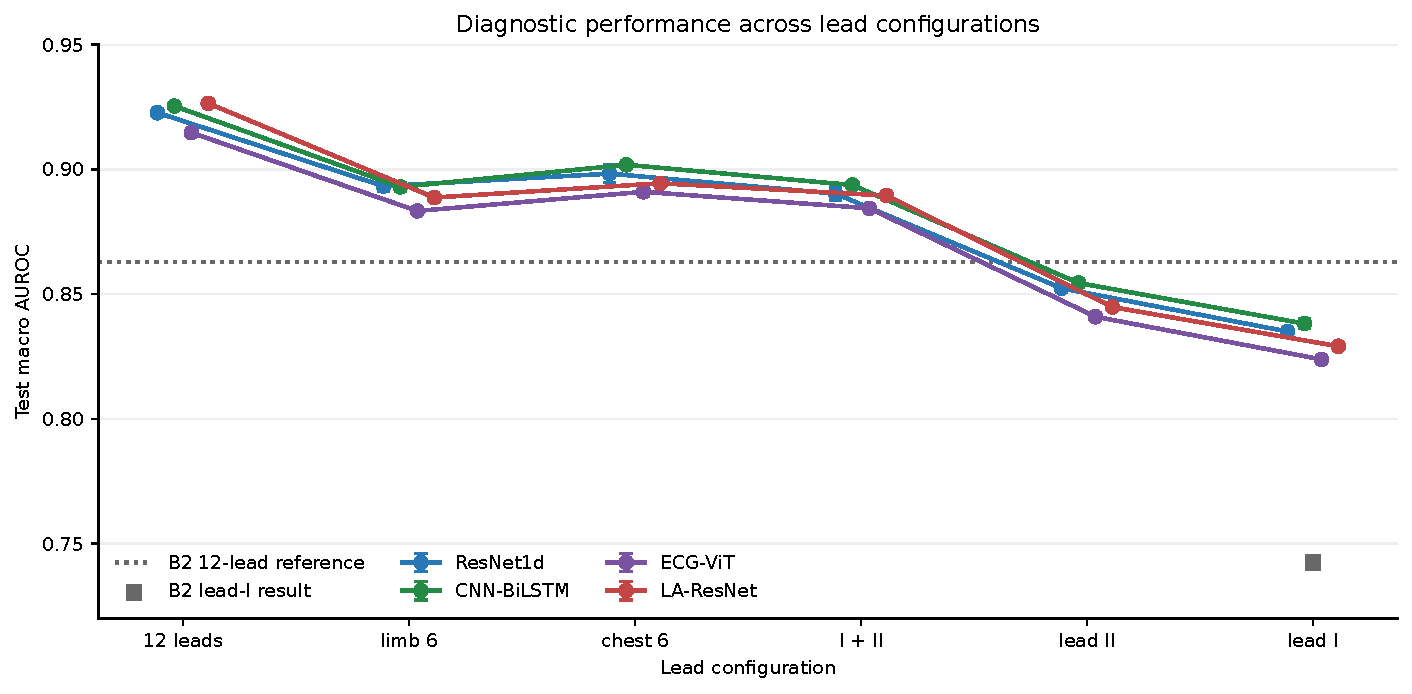
\includegraphics[width=0.92\linewidth]{figB_lead_ladder.pdf}
\caption{Test macro AUROC (mean $\pm$ SD over three seeds) across lead configurations for the three architectures trained from scratch and the single LA-ResNet model. The dotted line is the B2 feature baseline on 12 leads; the square is B2 on lead I.}
\label{fig:ladder}
\end{figure}

\begin{figure}[t]
\centering
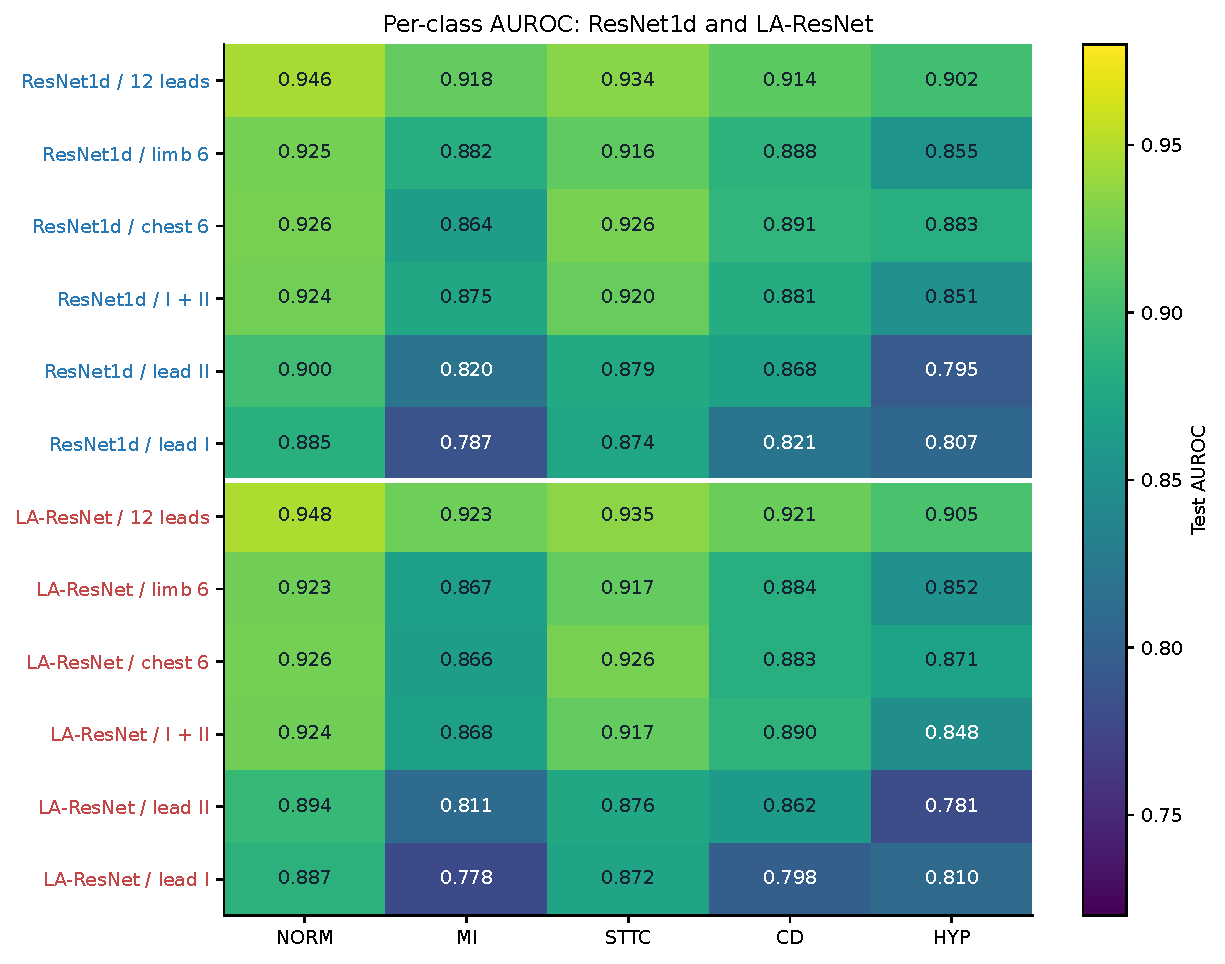
\includegraphics[width=0.72\linewidth]{figC_per_class_heatmap.pdf}
\caption{Per-class test AUROC (mean over three seeds) for dedicated ResNet1d models and the single LA-ResNet model across lead configurations.}
\label{fig:perclass}
\end{figure}

\subsection{Can a reduced lead set replace the 12-lead ECG?}
\label{sec:res_conclusion}
\Cref{fig:conclusion} applies the pre-specified criterion to every diagnosis and reduced configuration for the primary approach, CNN-BiLSTM, which was selected on the validation fold (its mean validation AUROC over the reduced configurations, 0.8866, was 0.0001 above that of ResNet1d). Of 30 cells (five diagnoses plus derived triage, times five configurations), 29 were \emph{not replaceable} and one met the \emph{screen} criterion: STTC with the six chest leads ($\Delta$AUROC $-0.004$ [$-0.010$, $+0.001$], \sensninety\ 0.84). This result did not depend on the choice of approach: STTC with chest6 was \emph{screen} for all five evaluated approaches ($\Delta$AUROC $-0.0045$ to $-0.0089$; lower CI bounds $-0.0097$ to $-0.0155$; \sensninety\ 0.82--0.84).

No diagnosis could be screened with lead I. The largest gap was MI ($\Delta$AUROC $-0.128$ [$-0.147$, $-0.107$], \sensninety\ 0.45), and even the derived triage score reached only 0.71 sensitivity at 90\% specificity. The verdicts were unchanged with a margin of 0.01. With a margin of 0.03, 8 of the 29 cells became \emph{conditional} (non-inferior AUROC but \sensninety\ $<0.80$) and none became \emph{screen}. The operating-point requirement is demanding: even the 12-lead CNN-BiLSTM reached a mean \sensninety\ of only about 0.74 for MI and 0.71 for HYP, so these classes could not have met the second condition with any input.

\begin{figure}[t]
\centering
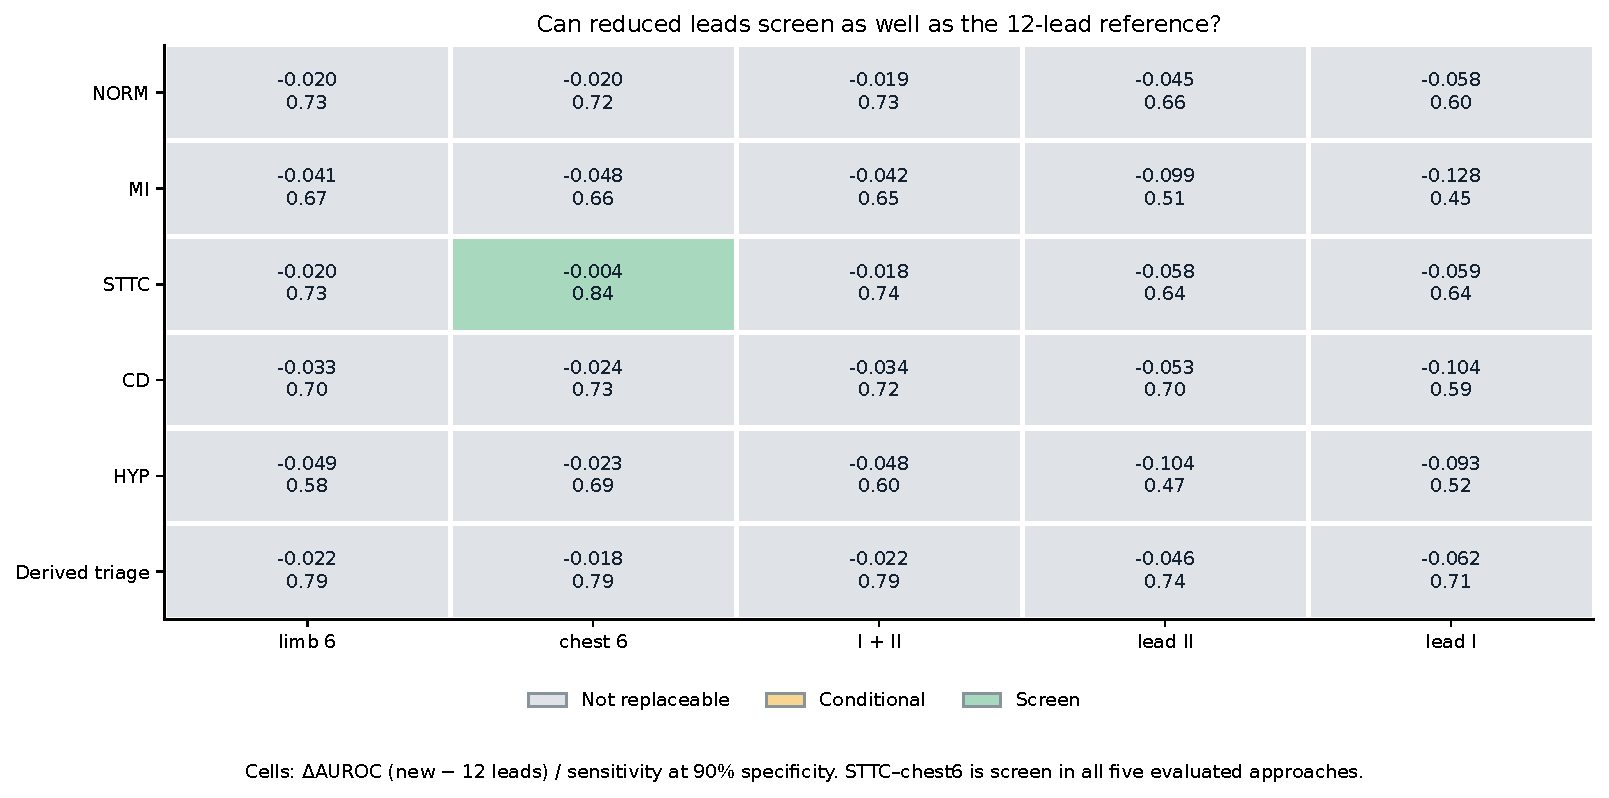
\includegraphics[width=\linewidth]{figD_conclusion_matrix.pdf}
\caption{Conclusion matrix for the validation-selected primary approach (CNN-BiLSTM). Each cell gives $\Delta$AUROC versus the 12-lead reference and the sensitivity at 90\% specificity; the colour gives the pre-specified verdict. STTC with the six chest leads is the only \emph{screen} cell and is \emph{screen} for all five evaluated approaches.}
\label{fig:conclusion}
\end{figure}

\subsection{Do training strategies recover the loss?}
Neither strategy recovered the information lost with the leads (\cref{tab:strategies}, \cref{fig:ladder}). Supervised transfer from the 12-lead ResNet1d changed the seed-ensemble AUROC by between $-0.0023$ and $+0.0022$ across the five configurations, with no comparison significant after Holm correction; freezing the backbone was worse than training from scratch with lead I ($-0.0078$ [$-0.0117$, $-0.0037$]).

A single LA-ResNet checkpoint served all six configurations. With 12 leads its mean AUROC (0.9264 $\pm$ 0.0004) was at least as high as that of the dedicated ResNet1d (0.9227 $\pm$ 0.0015). On reduced configurations it was 0.0033--0.0095 below the five dedicated scratch models, significantly so for chest6, lead II and lead I. The lead-agnostic design thus trades a small, measurable loss for the convenience of one model that accepts any of the six lead sets.

\begin{table}[t]
\centering
\small
\begin{threeparttable}
\caption{Training strategies versus dedicated ResNet1d trained from scratch: paired seed-ensemble $\Delta$AUROC (T1).}
\label{tab:strategies}
\begin{tabular}{llccc}
\toprule
Configuration & Strategy & $\Delta$AUROC & 95\% CI & Holm $p$ \\
\midrule
limb6 & S2 fine-tune & $-0.0003$ & [$-0.0031$, $+0.0025$] & 1.000 \\
 & S3 LA-ResNet & $-0.0044$ & [$-0.0079$, $-0.0011$] & 0.064 \\
chest6 & S2 fine-tune & $+0.0022$ & [$-0.0007$, $+0.0050$] & 0.732 \\
 & S3 LA-ResNet & $-0.0054$ & [$-0.0092$, $-0.0018$] & 0.018 \\
2lead & S2 fine-tune & $+0.0011$ & [$-0.0017$, $+0.0041$] & 1.000 \\
 & S3 LA-ResNet & $-0.0033$ & [$-0.0070$, $+0.0002$] & 0.462 \\
leadII & S2 fine-tune & $-0.0017$ & [$-0.0052$, $+0.0018$] & 1.000 \\
 & S3 LA-ResNet & $-0.0095$ & [$-0.0148$, $-0.0045$] & $<$0.001 \\
leadI & S2 fine-tune & $-0.0023$ & [$-0.0052$, $+0.0006$] & 0.732 \\
 & S2 frozen & $-0.0078$ & [$-0.0117$, $-0.0037$] & $<$0.001 \\
 & S3 LA-ResNet & $-0.0080$ & [$-0.0124$, $-0.0034$] & $<$0.001 \\
\bottomrule
\end{tabular}
\begin{tablenotes}\footnotesize
\item Holm adjustment covers all 29 paired comparisons (architectures, lead sets, strategies). $p<0.001$ is the resolution of 1,000 bootstrap resamples.
\end{tablenotes}
\end{threeparttable}
\end{table}

\subsection{Robustness, label efficiency and self-supervised pre-training}
\paragraph{Noise.} With 12 leads, all architectures degraded gracefully down to 5\,dB (\cref{fig:noise}). With lead I, severe noise changed the ranking: at 0\,dB the three-seed mean AUROC was 0.759 for ResNet1d but 0.686 for CNN-BiLSTM, although CNN-BiLSTM had been slightly better on clean signals (0.838 versus 0.835). This is a descriptive comparison under synthetic white noise.

\paragraph{Label efficiency.} With 12 leads, training on 10\% of the patients (1,681 records) cost 0.040 AUROC relative to the full training set (ResNet1d seed 0: 0.881 versus 0.921). With lead I, the same reduction cost only 0.023 (0.812 versus 0.835), and even the 10\%-data 12-lead model (0.881) outperformed the full-data lead-I model by 0.047 (\cref{fig:labels}). The single-lead gap is therefore limited mainly by the information in the input rather than by the amount of training data.

\paragraph{Self-supervised pre-training (E8).} Masked signal modelling improved ECG-ViT trained on 10\% of the labels (\cref{tab:ssl}): the seed-ensemble AUROC rose by $+0.0065$ [$+0.0020$, $+0.0112$] with 12 leads and by $+0.0149$ [$+0.0091$, $+0.0210$] with lead I (both significant after Holm correction for the two comparisons), and the across-seed SD fell from 0.0078 to 0.0006 (12 leads) and from 0.0026 to 0.0005 (lead I). Both pre-training runs reached the 100-epoch limit (best epochs 98 and 96), so convergence was not established and the gain is best read as a lower bound. Pre-training narrowed, but did not reverse, ECG-ViT's low-label disadvantage: its 10\%-label mean AUROC (0.876 with 12 leads, 0.810 with lead I) was comparable to, not better than, ResNet1d trained from scratch on 10\% of the labels (seed 0: 0.881 and 0.812).

\begin{figure}[t]
\centering
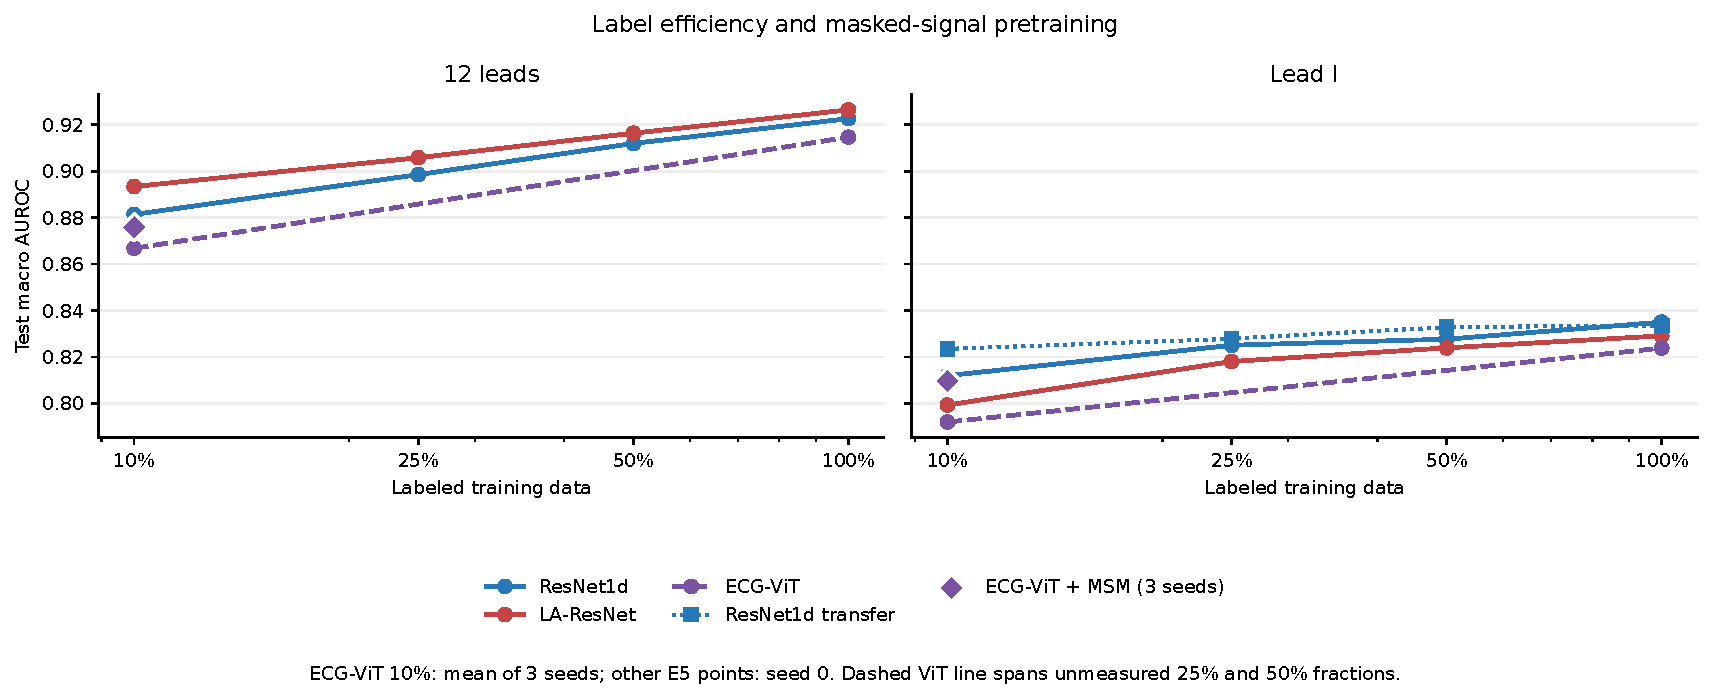
\includegraphics[width=\linewidth]{figE_label_efficiency.pdf}
\caption{Label efficiency with 12 leads and lead I. Points are seed 0 except ECG-ViT at 10\% (mean of three seeds); diamonds show ECG-ViT with masked-signal pre-training. Dashed lines span unmeasured fractions.}
\label{fig:labels}
\end{figure}

\begin{table}[t]
\centering
\small
\caption{Masked-signal pre-training (MSM) versus training from scratch for ECG-ViT with 10\% of the labels: three-seed mean $\pm$ SD and seed-ensemble AUROC [95\% CI]; paired difference on seed-ensemble predictions. The full-data ECG-ViT is a reference only.}
\label{tab:ssl}
\begin{tabular}{lcccc}
\toprule
Leads & Scratch & MSM & MSM $-$ scratch [95\% CI] & Full-data ViT \\
\midrule
12lead & \makecell{0.8668 $\pm$ 0.0078\\0.8860 [0.8771, 0.8955]} & \makecell{0.8759 $\pm$ 0.0006\\0.8924 [0.8837, 0.9012]} & \makecell{$+0.0065$ [$+0.0020$, $+0.0112$]\\$p=0.006$} & 0.9221 \\
\addlinespace
leadI & \makecell{0.7919 $\pm$ 0.0026\\0.8053 [0.7938, 0.8185]} & \makecell{0.8096 $\pm$ 0.0005\\0.8203 [0.8087, 0.8318]} & \makecell{$+0.0149$ [$+0.0091$, $+0.0210$]\\$p<0.001$} & 0.8287 \\
\bottomrule
\end{tabular}
\end{table}

\begin{figure}[t]
\centering
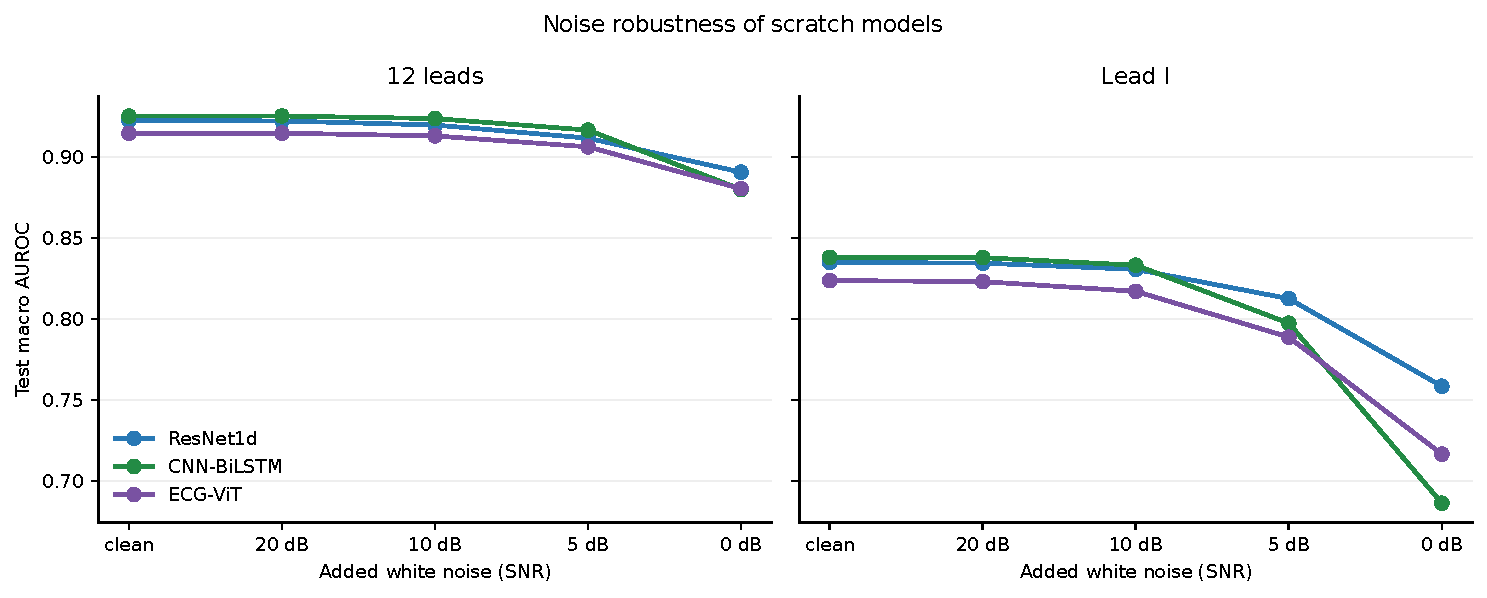
\includegraphics[width=0.7\linewidth]{figG_noise_robustness.pdf}
\caption{Test macro AUROC under additive white noise at test time, for 12 leads and lead I (three-seed means).}
\label{fig:noise}
\end{figure}

\subsection{Triage on PTB-XL and in an external hospital}
\label{sec:res_triage}
\paragraph{Internal triage.} Dedicated T2 models reached a seed-ensemble AUROC of 0.940 with 12 leads and 0.878 with lead I (ResNet1d); sensitivity at 90\% specificity fell from 0.83 to 0.71 (\cref{fig:triage}). A dedicated T2 model gave no apparent advantage over the derived score $1-P(\text{NORM})$ of T1 models (lead I: 0.705--0.708 versus 0.700--0.711). All reduced configurations were \emph{not replaceable} for triage; even the best, chest6 with LA-ResNet, narrowly missed both conditions ($\Delta$AUROC $-0.021$ [$-0.027$, $-0.015$], \sensninety\ 0.79).

\paragraph{External validation (E7).} Applied without retraining or re-tuning to 34,815 Chapman records, the frozen T2 models kept their discrimination (\cref{tab:external}, \cref{fig:triage}): ResNet1d reached 0.955 [0.953, 0.957] with 12 leads and 0.916 [0.913, 0.919] with lead I, compared with 0.940 and 0.878 on the PTB-XL test fold; LA-ResNet gave 0.957 and 0.912. The values depended on the label definition. Under the archived first mapping (v1) they were 0.953 and 0.910; when ``left ventricular high voltage''---a voltage criterion rather than a diagnosis of hypertrophy---was also counted as abnormal (v2 + LVHV), they fell to 0.936 and 0.880, close to the internal values. Across the three mappings, external AUROC ranged from 0.936 to 0.957 with 12 leads and from 0.875 to 0.916 with lead I.

Thresholds chosen on the PTB-XL validation fold for 90\% specificity transferred approximately but not exactly: on the external cohort they gave a sensitivity/specificity of 0.905/0.864 with 12 leads and 0.797/0.903 with lead I (ResNet1d). Because the external target is restricted (strictly sinus-rhythm negatives, mapped diagnoses only) and the case mix differs, the higher external AUROC should not be read as better generalisation, and it does not change the lead-I verdicts of \cref{sec:res_conclusion}, which are defined on PTB-XL.

\begin{figure}[t]
\centering
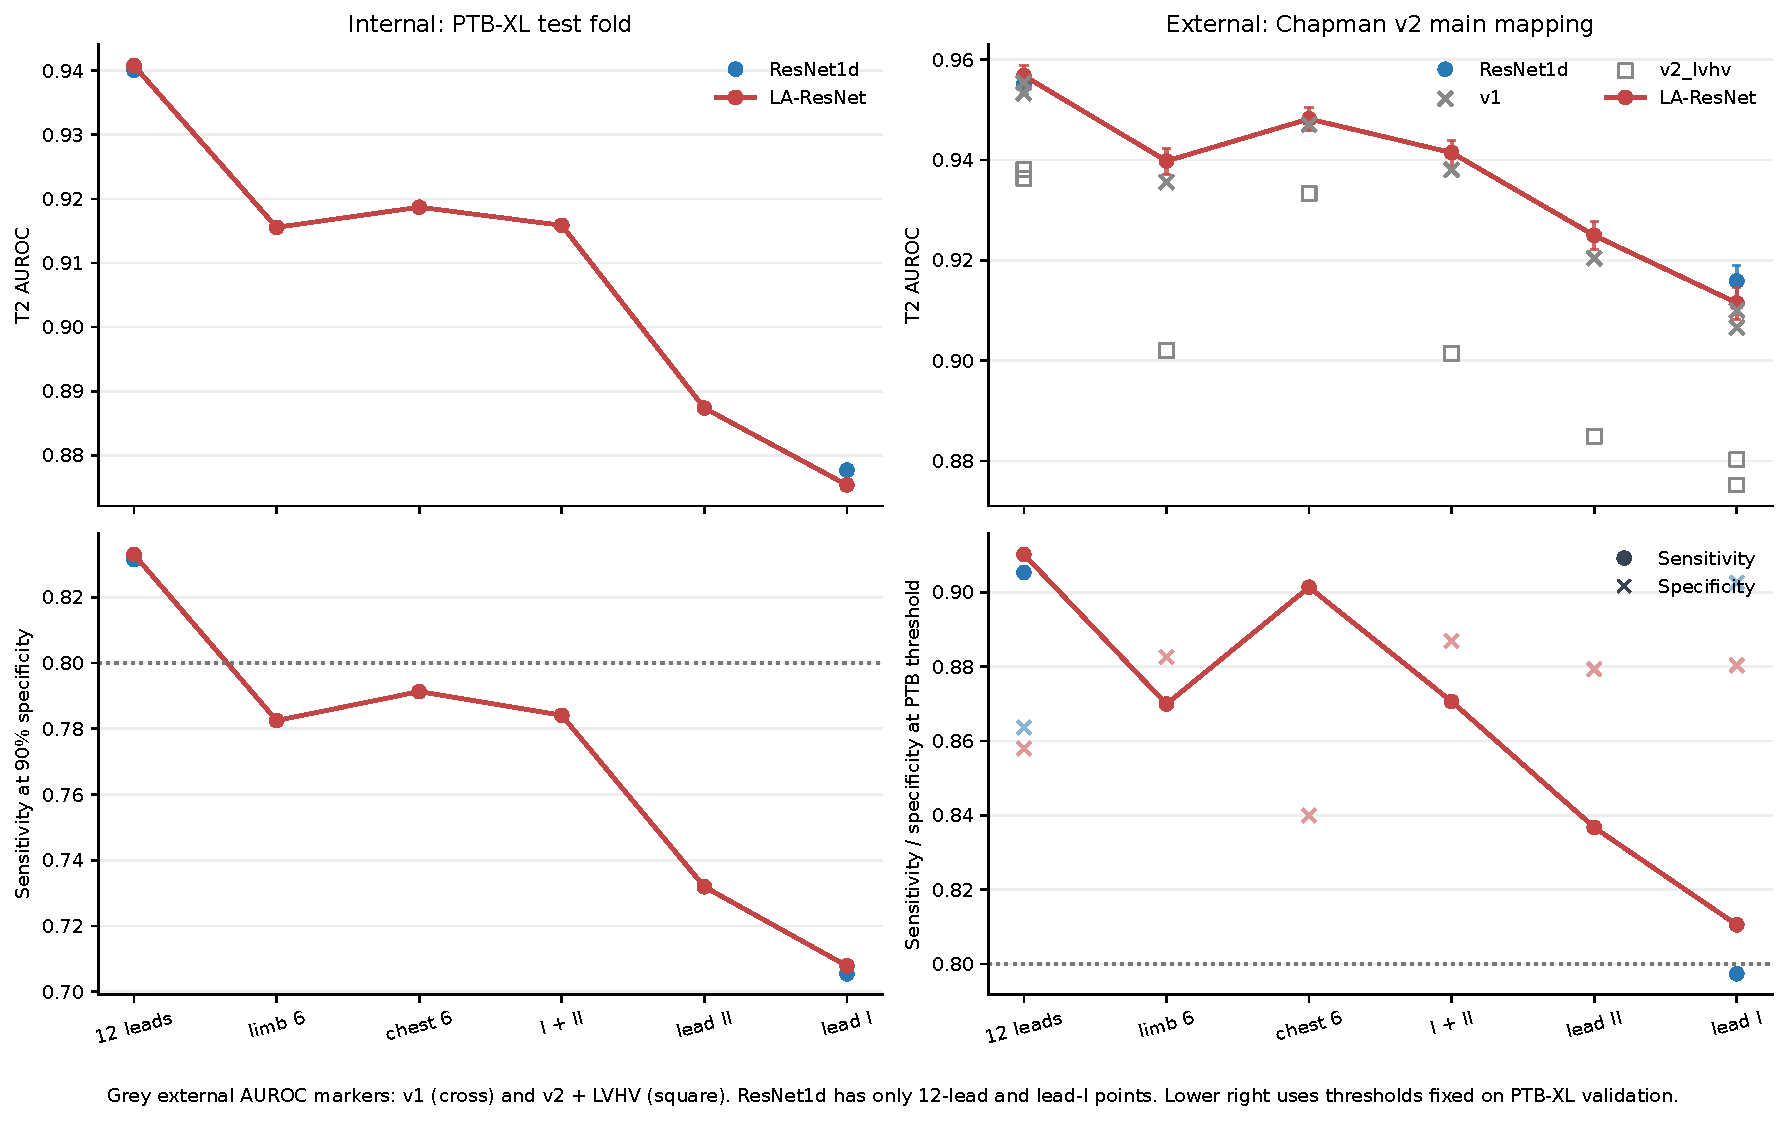
\includegraphics[width=\linewidth]{figF_triage_external.pdf}
\caption{Triage (T2). Left: PTB-XL test fold. Right: Chapman external cohort under the v2 mapping, with v1 and v2 + LVHV as sensitivity analyses (grey markers). Lower right: sensitivity and specificity at thresholds fixed on the PTB-XL validation fold.}
\label{fig:triage}
\end{figure}

\begin{table}[t]
\centering
\small
\caption{External validation of frozen T2 models on the Chapman cohort under three label mappings (v2 = main analysis). Sens/spec: sensitivity and specificity at the threshold chosen for 90\% specificity on the PTB-XL validation fold. The negative set (strictly sinus-rhythm records) is identical across mappings, so specificity at the transported threshold does not change; LA-ResNet under v1 and v2 + LVHV is listed in the results files.}
\label{tab:external}
\setlength{\tabcolsep}{4pt}
\resizebox{\linewidth}{!}{%
\begin{tabular}{lllcccc}
\toprule
Mapping & Model & Leads & $n$ (pos.) & External AUROC [95\% CI] & Internal AUROC & Sens/spec at PTB thr. \\
\midrule
v2 & ResNet1d & 12lead & 34,815 (16,092) & 0.955 [0.953, 0.957] & 0.940 & 0.905 / 0.864 \\
v2 & ResNet1d & leadI & 34,815 (16,092) & 0.916 [0.913, 0.919] & 0.878 & 0.797 / 0.903 \\
v2 & LA-ResNet & 12lead & 34,815 (16,092) & 0.957 [0.955, 0.959] & 0.941 & 0.910 / 0.858 \\
v2 & LA-ResNet & leadI & 34,815 (16,092) & 0.912 [0.908, 0.915] & 0.875 & 0.811 / 0.880 \\
\midrule
v1 & ResNet1d & 12lead & 31,364 (12,641) & 0.953 [0.951, 0.956] & 0.940 & 0.901 / 0.864 \\
v1 & ResNet1d & leadI & 31,364 (12,641) & 0.910 [0.907, 0.914] & 0.878 & 0.788 / 0.903 \\
v2+LVHV & ResNet1d & 12lead & 37,313 (18,590) & 0.936 [0.934, 0.939] & 0.940 & 0.851 / 0.864 \\
v2+LVHV & ResNet1d & leadI & 37,313 (18,590) & 0.880 [0.877, 0.884] & 0.878 & 0.728 / 0.903 \\
\bottomrule
\end{tabular}}
\end{table}

\subsection{Ensembles, uncertainty, subgroups and interpretability}
Averaging the three seeds improved the macro AUROC in all 38 model--configuration--task combinations (mean gain $+0.0045$). A heterogeneous ensemble of the three architectures reached 0.932 with 12 leads and 0.842 with lead I, only marginally above the best seed ensemble. Inter-model disagreement flagged harder records: among the 20\% of test records on which the models disagreed most, the label error rate was 0.196 versus 0.087 for the remaining records with 12 leads ($2.3\times$) and 0.256 versus 0.141 with lead I ($1.8\times$). Disagreement could therefore be used to refer uncertain recordings for review, although we did not test such a referral policy.

Subgroup AUROCs were broadly similar (for example, lead-I CNN-BiLSTM 0.846 in 1,110 male and 0.835 in 1,048 female records; \cref{app:subgroups}); without subgroup confidence intervals these estimates are descriptive and do not establish a fairness difference.

Grad-CAM maps of ResNet1d were broad and covered most of the recording (\cref{fig:explain}). This is expected: the receptive field of the last block (1,291 samples) exceeds the input length, so the maps indicate coarse regions rather than individual waves. The ECG-ViT attention matrix showed a strong vertical stripe at one key token (around 4.8--5.0\,s), a pattern consistent with an attention sink, to which we do not assign a physiological meaning. These visualisations are illustrative and are not causal clinical explanations.

\begin{figure}[t]
\centering
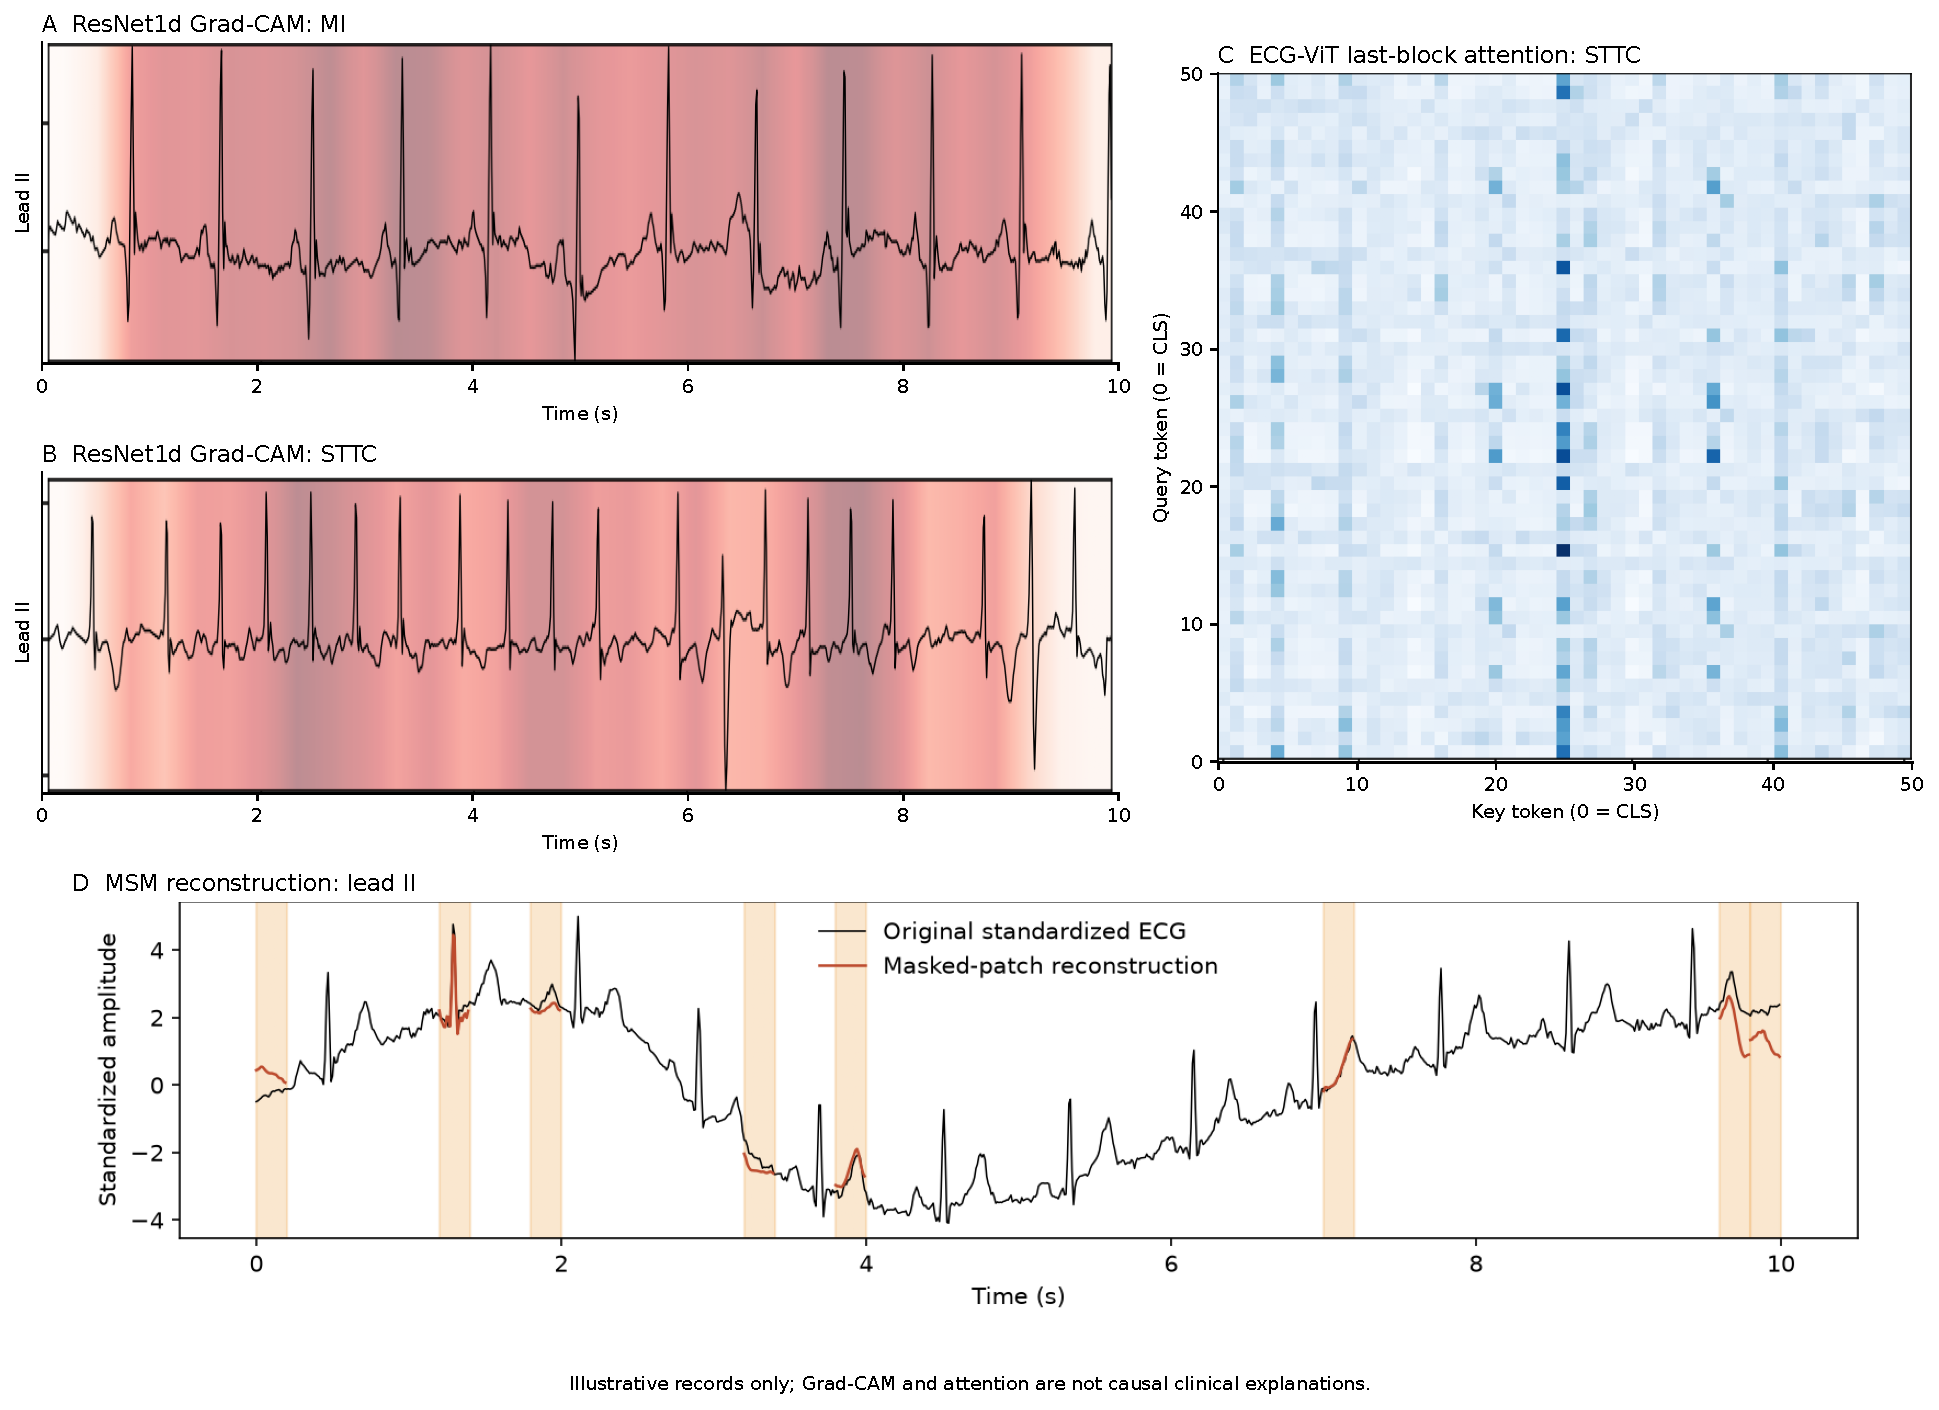
\includegraphics[width=\linewidth]{figH_explainability.pdf}
\caption{Illustrative explanations: ResNet1d Grad-CAM for MI and STTC (lead II), ECG-ViT last-block attention for an STTC record, and a masked-signal reconstruction example (shaded patches were hidden).}
\label{fig:explain}
\end{figure}
